\section{Descripci\'on de la Clase}
\subsection{Sumario}
\noindent \textbf{Objetivo}: Hacer una descripi\'on de la estructura de datos \textit{Segment Tree}.\\
\noindent \textbf{M\'etodo:} Expositivo-Ilustrativo.\\
\noindent \textbf{Medios:} Voz, Pizarra, Entorno de Desarrollo Integrado (IDE).\\

\noindent \textbf{Contenido:}\\
\begin{itemize}
    \item Necesidad del uso de la Estructura.
    \item Presentaci\'on de la Estructura.
    \item Construcci\'on de un Segment Tree.
    \item Consultas en Rangos.
    \item Actualizaciones de Posici\'on.
    \item Aplicaciones.
\end{itemize}


\section{El problema}
\subsection{Motivaci\'on}
Supongamos que se nos da un arreglo \texttt{A} de largo $n$. Ahora nos dan dos enteros $a$ y $b$ y nos piden calcular la suma de los elementos en el subarreglo desde la posici\'on $a$ hasta la posici\'on $b$, o sea, la suma de los elementos del arreglo en el rango $[a, b]$.

La soluci\'on ser\'ia recorrer los elementos del arreglo \texttt{A} que est\'an entre las posiciones $a$ y $b$, y acumular su suma. La complejidad temporal de este procedimiento ser\'ia $O(n)$, en el peor caso. 

Pero que pasar\'ia si, dado el arreglo, en vez de preguntarnos una vez la suma de un rango, nos hicieran $m$ preguntas con rangos diferentes. La complejidad temporal necesaria para responder las $m$ preguntas ser\'ia $O(n \cdot m)$.

Vamos a tratar de responder las $m$ preguntas m\'as r\'apido, o sea, en una complejidad menor que $O(n \cdot m)$.


\section{La Estructura de Datos}
\subsection{Introducci\'on a la Estructura}
Un \textit{segment tree}, o \'arbol de segmentos, es una estructura de datos que permite responder a consultas en rangos de forma r\'apida. Por ejemplo, nos permite calcular cu\'al es el m\'inimo en un rango, o cu\'al es la suma de los elementos de un rango, en un tiempo proporcional a $O(\log n)$.

Adem\'as, la estructura es capaz de actualizar un elemento del arreglo y luego seguir respondiendo consultas en rangos. A la ope\-ra\-ci\'on de actualizar un elemento en una posici\'on, se le conoce como \textit{point update} o actualizaci\'on de posici\'on.\\

\noindent Tipo de Datos Abstracto \textit{Segment Tree}:
%~ Tabla
        \begin{center}
        
        \begin{tabular}{|p{2.0cm}|p{4cm}|p{1.8cm}|}    
        
        \hline
        
        Operaci\'on &
        Descripci\'on &
        Complejidad \\
            
        \hline
        
        Construcci\'on{} & 
        Se construye el Segment Tree a partir de un arreglo inicial. &
        $O(n)$\\
        
        \hline
        
        Consulta en Rango &
        
        Se calcula el resultado de la consulta en rango. Por ejemplo, el m\'inimo, la suma, etc. &
        
        $O(\log n)$ \\
        
        \hline
        
        Actualizaci\'on de posici\'on &
        Se actualiza el valor de una posici\'on. &
        $O(\log n)$ \\
        
        \hline
            
        \end{tabular}    
        \end{center}

\subsection{Descripci\'on de un Segment Tree}
Un segment tree es una estructura en forma de \'arbol. Especificamente es un \'arbol binario, o sea, cada v\'ertice puede tener a lo m\'as dos hijos.

Cada nodo guarda un resultado precalculado para un rango del arreglo.  

Supongamos que nos dan un arreglo $a$ con los elementos $\{2, 3, 1, 6, 2, 1\}$ (comenzamos los \'indices desde el $1$ para mayor comodidad) y nos piden responder para cada consulta, la suma en el rango. Vamos a construir un segment tree para ese arreglo.

El valor correspondiente a la ra\'iz del \'arbol es la suma de los elementos del arreglo completo. El valor del hijo izquierdo de la ra\'iz es igual a la suma de los tres primeros elementos del arreglo. Igualmente, el valor del hijo derecho es igual a la suma de los tres \'ultimos elementos del arreglo.

En general, para cada nodo que no es hoja, si su rango es $[l, r]$, entonces el rango de su hijo izquierdo es $[l, m]$ y el de su hijo derecho es $[m+1, r]$, donde $m = \frac{l+r}{2}$.

Observe en la figura que el nodo correspondiente al rango $[1, 3]$ tiene un resultado igual a $6$ (que es la suma de los elementos en el rango) y que el resultado de su hijo izquierdo es $5$ y el de su hijo derecho es $1$.

Si el nodo es una hoja, su rango cubre solo un elemento del arreglo, por lo que su resultado puede calcularse inmediatamente y es igual al valor de dicho elemento.

\begin{minipage}{\columnwidth}
    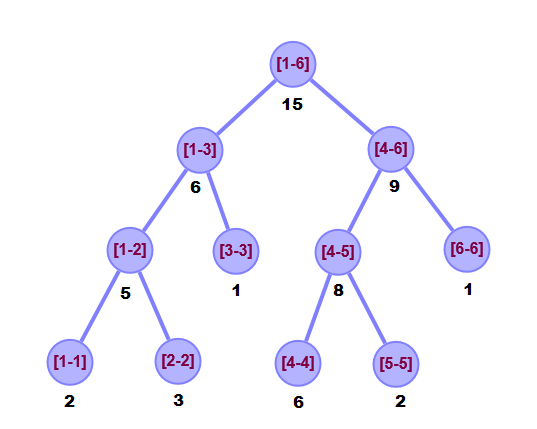
\includegraphics[width=\linewidth]{imag/segment_tree_suma.png}
    \label{example_sum}
\end{minipage}

Si nos pidieran calcular la suma de los elementos en el rango $[1, 5]$, lo cual es una consulta de rango, podemos obtener la res\-pues\-ta sin tener que recorrer todas las posiciones. Observe que podemos sumar los resultados de los nodos correspondientes a los rangos $[1, 3]$ y $[4, 5]$. Como vemos en la figura:

\begin{minipage}{\columnwidth}
    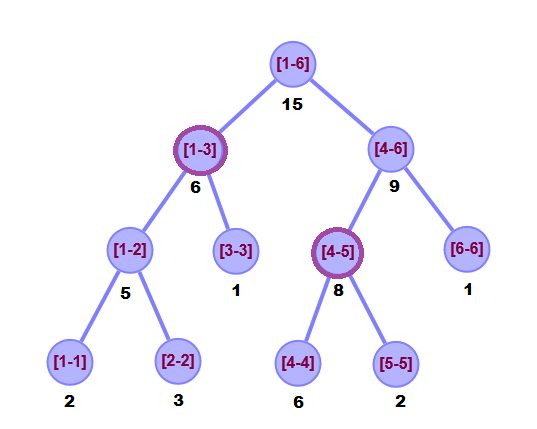
\includegraphics[width=\linewidth]{imag/segment_tree_query.png}
    \label{example_query}
\end{minipage}

Esa es la idea detr\'as de muchas estructuras de datos y especialmente del segment tree: precalculamos algunos valores que nos permiten luego obtener los resultados en menor tiempo. 

\hfill \break
\textit{?`Cu\'antos nodos puede tener un segment tree?}

Si construimos un segment tree para un arreglo de $n$ elementos, siendo $n$ igual a una potencia de $2$ ($n = 2^k$), el primer nivel del \'arbol, que es el de la ra\'iz, contiene un nodo ($2^0$ nodos); el segundo nivel tiene dos nodos ($2^1$ nodos), el tercer nivel tiene $2^2$ nodos y asi sucesivamente hasta el nivel que est\'a formado por las hojas, que son $2^k$.

El total de nodos ser\'a entonces:
$$ 2^0 + 2^1 + 2^2 + \cdots + 2^k = 2^{k+1} - 1 = 2 \cdot 2^k - 1$$

pero como $n = 2^k$, entonces el total de v\'ertices es $2 \cdot n-1$.

Si $n$ no fuera igual a una potencia de $2$, podemos agregar posiciones al final del arreglo hasta que $n$ sea igual a una potencia de $2$ y conseguir\'iamos el mismo resultado. 

\begin{property}
    La cantidad de v\'ertices m\'axima de un segment tree construido para un arreglo de largo $n$ es igual a $2\cdot n - 1$.
\end{property}

\hfill \break
\textit{?`Cu\'al es la altura m\'axima que puede tener un segment tree?}
Supongamos otra vez que construimos un segment tree para un arreglo de $n$ elementos, siendo $n$ igual a una potencia de $2$ ($n = 2^k$). El \'arbol tiene $k+1$ niveles (numerados desde $0$ hasta $k$). Pero como $n = 2^k$, entonces $k = \log_2(n)$; por lo que la altura del \'arbol ser\'a igual a $\log_2(n) + 1$.

\begin{property}
    La altura de un segment tree construido para un arreglo de largo $n$ es a lo m\'as $\log_2(n) + 1$.
\end{property}
\subsection{Construcci\'on de un Segment Tree}
Antes de construir un segment tree, debemos decidir dos cosas:
\begin{itemize}
    \item{
        El \textit{valor} que se guarda en cada nodo. Por ejemplo, para un
        segment tree de suma, guardamos la suma en el rango correspondiente al nodo.
    }
    \item{
        La operaci\'on que mezcla dos nodos hijos para obtener el resultado del
        nodo padre. En el caso de la suma, se puede simplemente sumar los resultados de los hijos
        para obtener la suma en el padre.
    }
\end{itemize}

Decidir estos dos elementos puede parecer trivial pero, en usos m\'as avanzados de la
estructura, no lo es.

Para construir el segment tree utilizamos una funci\'on recursiva \texttt{build()},
comenzamos en la ra\'iz del arbol (nodo $1$ en el arreglo).
Si el intervalo del nodo actual cubre m\'as de un elemento, entonces podemos calcular su resultado
como la combinaci\'on de los resultados de sus hijos (en el caso del segment tree de suma, la suma;
en el de m\'inimo, el m\'inimo de los dos resultados de los hijos). Ahora llamamos recursivamente a
la funci\'on \texttt{build()} para calcular el resultado de los hijos. Si llegamos a un nodo cuyo
intervalo solo contiene una posicion (un nodo hoja), directamente le asignamos el resultado al nodo
y lo devolvemos.

La complejidad temporal de este procedimiento es $O(n)$. Cada nodo se visita una vez y la cantidad
de nodos en el segment tree es a lo m\'as $2\cdot n -1$.

\subsection{Consultas en Rangos}
Vamos a analizar el caso de las consultas en rango para un segment tree de suma. Recibimos dos enteros $a$ y $b$ que representan los l\'imites del rango al que hay que calcularle la suma en un tiempo proporcional a $O(\log n)$.

\begin{corollary}[Consulta en Rangos]

    Nuestro pro\-ce\-di\-mien\-to es recursivo. Comenzamos en el v\'ertice ra\'iz. Cuando llegamos a un nodo $v$ cuyo rango es $[l, r]$, tenemos tres casos posibles:

    \begin{enumerate}
        \item{
            \textit{Si el intervalo $[l, r]$ del nodo est\'a completamente DENTRO del intervalo $[a, b]$:} Se retorna el resultado co\-rres\-pon\-dien\-te al v\'ertice actual (en este caso la suma), ya que este resultado debe ser tomado en cuanta para calcular la respuesta final.
        }
        \item{
           \textit{Si el intervalo $[l, r]$ del nodo est\'a completamente FUERA del intervalo $[a, b]$:} Se retorna un valor que no modifique la respuesta final. Como estamos calculando la suma, este valor es el cero.
        }
        \item{
            \textit{Si no se cumple NINGUNA de las condiciones anteriores:} Entonces llevamos a cabo este procedimiento en los hijos del nodo actual y luego combinamos la respuesta de cada ve\'rtice hijo, de ah\'i la naturaleza recursiva de este algoritmo.
        }
    \end{enumerate}

\end{corollary}



Para el ejemplo del arreglo $\{2, 3, 1, 6, 2, 1\}$, y la consulta de la suma del rango $[1, 5]$, comenzar\'iamos en el nodo del intervalo $[1, 6]$. Este nodo no cumple ninguna de los dos primeros casos, por lo que aplicando el tercero, llamamos a la funci\'on recursivamente en sus hijos.

\begin{minipage}{\columnwidth}
    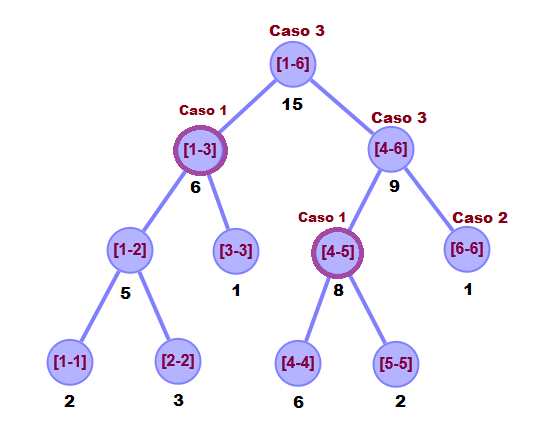
\includegraphics[width=\linewidth]{imag/segment_tree_query_casos}
    \label{fig:example_st_casos}
\end{minipage}

Para el hijo izquierdo, correspondiente al intervalo $[1, 3]$ se cumple la primera regla, porque el intervalo del nodo est\'a completamente dentro del intervalo de la consulta. Entonces retornamos el resultado precalculado de este v\'ertice. En este caso no hacemos m\'as llamadas recursivas en los hijos de este nodo.

El hijo derecho de la ra\'iz solo cumple la regla $3$, por lo que aplicamos el procedimiento a sus hijos. Para el nodo correspondiente al intervalo $[4, 5]$ se cumple la regla $1$. Entonces retornamos su valor precalculado. Para el nodo del rango $[6, 6]$ se cumple la regla $2$, por lo que devolvemos un valor que no modifique la respuesta; en este caso ese valor es el cero. 


Vamos a repasar los valores que obtuvimos en cada nodo: En el nodo del intervalo $[1, 3]$ obtuvimos el valor $6$. En el nodo del intervalo $[4, 5]$ obtuvimos el valor $8$ y en el nodo del intervalo $[6, 6]$, el valor cero. La suma de estos valores es la respuesta a la consulta: $6 + 8 + 0 = 14$.

Hay que aclarar que \textbf{los valores que se calculan para cada nodo en las consultas en rangos no modifican los valores del segment tree}, sino que son valores temporales que sirven para obtener el resultado de la consulta. \\

\begin{minipage}{\columnwidth}
    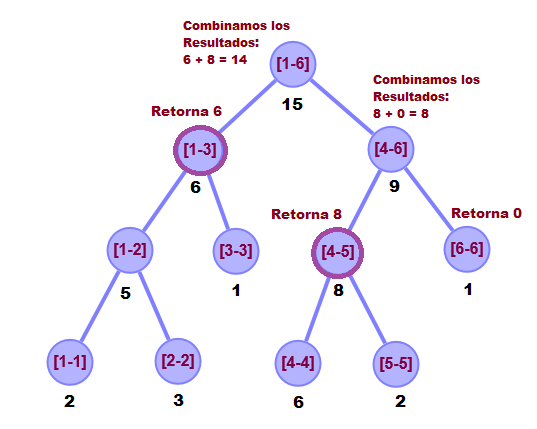
\includegraphics[width=\linewidth]{imag/segment_tree_query_values}
    \label{fig:example_st_casos}
\end{minipage}

\noindent\textit{?`Cu\'al es la complejidad temporal de una consulta en rangos?}\\
En este caso la complejidad temporal depende de la cantidad de nodos que son visitados durante la consulta. Una observaci\'on necesaria, es que en cada nivel del \'arbol visitamos a lo m\'as 4 v\'ertices. Este hecho puede probarse mediante inducci\'on, pero no lo vamos a hacer aqu\'i. 

Si en cada nivel visitamos a lo m\'as  cuatro nodos, y el segment tree tiene a lo m\'as $\log_2(n) + 1$ niveles (porque su altura es a lo m\'as $\log_2(n) + 1$), entonces vamos a visitar en total de $4 \cdot \log_2(n) + 4$ v\'ertices en el peor caso. La complejidad final es $O(\log n)$.
\subsection{Actualizaciones de Posici\'on}
Ahora se necesita modificar un elemento del arreglo \texttt{A} original y seguir contestando consultas en rangos. Se obtiene un nuevo arreglo \texttt{A'} que difiere del original solo en una posici\'on.

Deseamos obtener un segment tree para el arreglo \texttt{A'}, pero sin construirlo desde cero, en vez de eso, vamos a utilizar el segment tree ya existente. Debemos modificar nuestra estructura de tal manera que los resultados que precalculamos para cada nodo sean los correspondientes al nuevo arreglo \texttt{A'}. A esta operaci\'on se le conoce como actualizaci\'on de posici\'on.\\

\noindent\textit{?`Cu\'ales son los nodos cuyo valor hay que modificar?} \\
Primeramente si $p$ es la posici\'on que vamos a modificar, entonces debemos actualizar el valor del nodo hoja cuyo intervalo es $[p, p]$, porque su valor depende totalmente del n\'umero en la posici\'on $p$ del arreglo. Pero cuando construimos el segment tree original, el valor del padre de ese nodo fue calculado como la suma de los valores de dicho nodo y el otro hijo, por lo que si modificamos el valor del nodo, hay que modificar el valor del padre.

Pero lo mismo pasa con el padre del padre, y con el siguente nodo en direcci\'on a la ra\'iz... En conclusi\'on, se modifica el v\'ertice $v$, cuyo rango es $[p, p]$, y todos los dem\'as nodos en el camino entre $v$ y la ra\'iz del \'arbol.

Por ejemplo, si vamos a modificar la posici\'on $p = 3$ y le vamos a colocar el valor $5$, modificamos el nodo de rango $[3, 3]$ que antes ten\'ia el valor $1$, ahora le colocamos el valor $5$. Luego actualizamos el valor del nodo de rango $[1, 3]$. Ahora ser\'a $5 + 5 = 10$. Por \'ultimo actualizamos el valor de la ra\'iz: $10 + 9 = 19$.

\begin{minipage}{\columnwidth}
    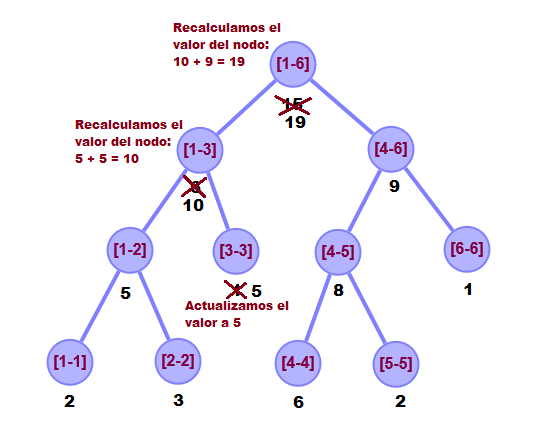
\includegraphics[width=\linewidth]{imag/segment_tree_update}
    \label{fig:example_st_casos}
\end{minipage}

Observe que el segment tree resultante es igual al segment tree que hubi\'esemos construido si el arreglo original fuera $\{2, 3, \underline{5}, 6, 2, 1\}$.

En el caso de la actualizaci\'on de posici\'on \textbf{los valores que se calculan para cada nodo en las actualizaciones s\'i modifican los valores de los nodos del segment tree}.

Ahora hay que formalizar el m\'etodo de la actualizaci\'on de posici\'on para posteriormente implementarlo. 

\begin{corollary}[Actualizaci\'on de Posici\'on]
    Nos dan una posici\'on $p$ a modificar, y un valor $x$ que es el nuevo valor. El procedimiento es recursivo y comienza en el nodo ra\'iz. Cuando llegamos a un v\'ertice $v$ cuyo rango es $[l, r]$ tenemos tres casos posibles:

    \begin{enumerate}
        \item{
            \textit{Si el intervalo $[l, r]$ del nodo est\'a completamente DENTRO del intervalo $[p, p]$ (Esto solo se cumple si $l = r = p$):}  Como $l = r = p$ entonces el nodo actual es el nodo hoja cuyo intervalo es $[p, p]$. El nuevo valor del nodo ser\'a $x$, el cual se retorna.
        }
        \item{
            \textit{Si el intervalo $[l, r]$ del nodo est\'a completamente FUERA del intervalo $[p, p]$:} No se modifica el nodo y se retorna el valor que ya ten\'ia.
        }
        \item{
            \textit{Si no se cumple NINGUNA de las condiciones anteriores:} Entonces llevamos a cabo este procedimiento en los hijos del nodo actual y luego combinamos la respuesta de cada v\'ertice hijo, para recalcular el valor del nodo actual con los valores retornados.
        }
    \end{enumerate}
\end{corollary}

\noindent\textit{?`Cuál es la complejidad temporal de una actualizaci\'on de posici\'on?} \\
Al igual que en los m\'etodos anteriores, la complejidad temporal depende de la cantidad de v\'ertices del \'arbol que ser\'an visitados. Como solo se modifican los nodos en el camino desde el vertice $v$ hasta la ra\'iz utilizando ambos hijos para recalcular los valores, en cada nivel del \'arbol se visitan a lo m\'as dos nodos. La cantidad de nodos total ser\'a como m\'aximo $2 \cdot \log_2(n) + 2 = O(\log n)$.



\subsection{Implementaci\'on}
Para representar el \'arbol del segment tree vamos a utilizar un arreglo \texttt{T}. El resultado del nodo ra\'iz se guarda en \texttt{T[1]}. En general, si el resultado de un nodo se guarda en la posici\'on $p$, entonces el resultado de su hijo izquierdo se guarda en la posici\'on $2 \cdot p$ y el resultado de su hijo derecho se guarda en $2 \cdot p + 1$. Esta representaci\'on es v\'alida para cualquier \'arbol binario. De esta forma podemos guardar el segment tree construido para un arreglo \texttt{A} de largo $n$ en un arreglo \texttt{T} de largo a lo m\'as $4n$. 

El segment tree para el arreglo original quedar\'ia guardado en el arreglo de la siguiente forma:

\begin{minipage}{\columnwidth}
    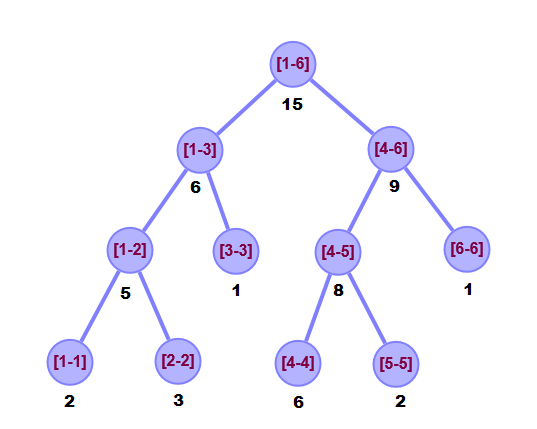
\includegraphics[width=\linewidth]{imag/segment_tree_suma}
    \label{example_st_casos}
\end{minipage}

\noindent \begin{minipage}{\linewidth}
    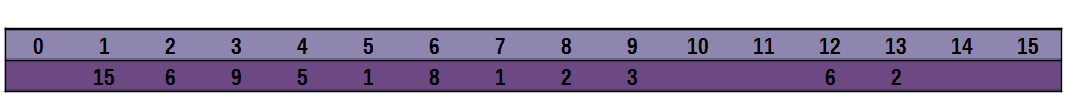
\includegraphics[width=\linewidth]{imag/arreglo2}
    \label{example_st_casos}
\end{minipage}

Creamos una clase \texttt{SegmentTree} que tiene como atributos al largo del arreglo \texttt{n}, al arreglo dado \texttt{A}, y al arreglo \texttt{T}, donde guardaremos los valores del \'arbol. El constructor de la clase inicializa los valores de los atributos y llama a la funci\'on \texttt{build()}.

\raggedbottom\lstinputlisting[style=java]{segment_tree_code/constructor.java}

El m\'etodo \texttt{build()} construye el segment tree. Recibe como par\'ametros \texttt{l} y \texttt{r}, que son los los extremos del rango del nodo y \texttt{nod} que es la posici\'on del nodo actual en el arreglo \texttt{T}. Inicialmente se llama a las funciones con \texttt{l = 1}, \texttt{r = n} y \texttt{nod = 1}, que son los valores correspondientes al v\'ertice ra\'iz.
  
Si el nodo actual es un nodo hoja (o sea, si \texttt{l == r}) entonces inicializamos el valor del nodo con el valor correspondiente del elemento del arreglo, que es \texttt{A[l]}.

Si no es as\'i preguntamos recursivamente los valores de los hijos y cuando estos sean respondidos, los combinamos y los guardamos como el valor del nodo.

Observe que en todos los m\'etodos calculamos el valor de \texttt{m} y llamamos a los hijos izquierdo y derecho con sus par\'ametros para \texttt{l}, \texttt{r} y \texttt{nod} correspondientes: \texttt{(l, m, 2*nod)} para el hijo izquierdo y \texttt{(m+1, r, 2*nod+1)} para el derecho.
\raggedbottom\lstinputlisting[style=java]{segment_tree_code/build.java}

El siguente m\'etodo es \texttt{query()}, correspondiente a la consulta en rango. Su versi\'on p\'ublica llama al m\'etodo privado. El privado recibe como argumentos a los extremos del rango de la consulta \texttt{a} y \texttt{b} adem\'as de los par\'ametros \texttt{l}, \texttt{r} y \texttt{nod}. Los primeros dos bloques \texttt{if} corresponden a los dos primeros casos del m\'etodo. Si el nodo no corresponde a ninguno de ellos, entonces preguntamos recursivamente a sus hijos, haciendo las llamadas con los par\'ametros correspondientes.

\raggedbottom\lstinputlisting[style=java]{segment_tree_code/query.java}

Por \'ultimo vamos a hablar del m\'etodo \texttt{update()} que lleva a cabo las actualizaciones de posici\'on. Este m\'etodo tiene tambi\'en su versi\'on p\'ublica.

Los primeros dos bloques \texttt{if} corresponden a los dos primeros casos del m\'etodo. Si el nodo no corresponde a ninguno de ellos, entonces preguntamos recursivamente a sus hijos, haciendo las llamadas con los par\'ametros correspondientes. Luego combinamos las respuestas, actualizamos los valores en el \'arbol y por \'ultimo retornamos el valor obtenido.


\raggedbottom\lstinputlisting[style=java]{segment_tree_code/update.java}

\section{Conclusiones}
\subsection{Ventajas y Aplicaciones}
Para resolver el problema de las consultas en rango con actualizaciones de posici\'on de forma ingenua, o sea recorriendo todos los elementos del rango en cada consulta se requiere un costo computacional mayor que para resolverlo con un segment tree. Pero ?`cu\'an grande es la mejora? 

Supongamos que el largo de nuestro arreglo es $n$ y que deseamos hacer $m$ operaciones, entre consultas y actualizaciosnes. Para que una computadora moderna pueda hacer todas las operaciones en un segundo, el producto $n \cdot m$ no puede ser mayor que $10^8$. Un posible caso ser\'ia $n = 10000$ y $m = 10000$. Estas cantidades son aproximadas y dependen del \textit{hardware} de la m\'aquina.

Usando un segment tree se pueden realizar en un segundo apro\-xi\-ma\-da\-men\-te $10^5$ operaciones en un arreglo de hasta un mill\'on de elementos. \\

\noindent \textit{?`Qu\'e m\'as podemos hacer con un segment tree?} \\
Esta estructura es muy flexible. Recordemos que lo que se puede hacer con ella depende de lo que guardemos en cada nodo y de la forma de combinar esos resultados. 

Existen aplicaciones donde se guarda en los nodos del segment tree un arreglo o un \'arbol binario como el AVL. Incluso en un nodo puede guardarse otro segment tree. 

Las aplicaciones b\'asicas incluyen responder el m\'aximo en un rango, m\'inimo, el m\'aximo com\'un divisor, la suma, el producto, entre otras. Pero existen aplicaciones en las que podemos responder cu\'antos elementos diferentes hay en un rango o cu\'al es la mayor subsecuencia creciente.

Incluso podemos responder consultas en un rango de dos dimensiones (o sea, un rect\'angulo) de una matriz. O hacer consultas en rango de una versi\'on vieja de un segment tree, despu\'es de haberlo modificado con varias actualizaciones de posici\'on. 

